\graphicspath{{images/}}

\section{Ход работы}

Я выбрал набор данных Smoker Condition \cite{kaggle} для выполнения лабораторной работы. Требуется предсказать, будет ли у человека рак лёгких, основываясь на его генетике и на том, курит ли он.

Признаки в наборе данных:

\begin{enumerate}
    \item
    Gene2337 --- результат количественного анализа Gene2337.
    \item
    Gene35715 --- результат количественного анализа Gene35715.
    \item
    Gene12936 --- результат количественного анализа Gene12936.
    \item
    Gene1689 --- результат количественного анализа Gene1689.
    \item
    FGFR1 --- результат количественного анализа FGFR1 (рецептор фактора роста фибробластов).
    \item
    GATA4 --- результат количественного анализа GATA4.
    \item
    type --- является ли человек курильщиком. В работе я переименовал признак в <<Is smoker?>> с числовым значением $0$ или $1$.
    \item
    Condition --- состояние лёгких человека. В работе я переименовал признак в <<Has cancer?>> с числовым значением $0$ или $1$.
\end{enumerate}

Перед выявлением зависимостей между признаками следует проверяю целостность набора данных:
\begin{alltt}
RangeIndex: 1023 entries, 0 to 1022
Data columns (total 8 columns):
 #   Column     Non-Null Count  Dtype
---  ------     --------------  -----
 0   Gene2337   1022 non-null   float64
 1   Gene35715  1020 non-null   float64
 2   Gene12936  1020 non-null   float64
 3   Gene1689   1020 non-null   float64
 4   FGFR1      1021 non-null   float64
 5   GATA4      1021 non-null   float64
 6   type       1023 non-null   object
 7   Condition  1023 non-null   object
dtypes: float64(6), object(2)
memory usage: 64.1+ KB
\end{alltt}

В наборе есть неполные данные, которые я удаляю. Категориальные признаки привожу к числовым, преобразую соответствующие столбцы с данными.

Данные после преобразования имеют следующий вид:
\begin{alltt}
Int64Index: 1000 entries, 0 to 1019
Data columns (total 8 columns):
 #   Column       Non-Null Count  Dtype
---  ------       --------------  -----
 0   Gene2337     1000 non-null   float64
 1   Gene35715    1000 non-null   float64
 2   Gene12936    1000 non-null   float64
 3   Gene1689     1000 non-null   float64
 4   FGFR1        1000 non-null   float64
 5   GATA4        1000 non-null   float64
 6   Is smoker?   1000 non-null   int64
 7   Has cancer?  1000 non-null   int64
dtypes: float64(6), int64(2)
memory usage: 102.6 KB
\end{alltt}
\pagebreak

Построю графики для каждой пары признаков. Синим отмечены нормальные лёгкие, оранжевым лёгкие с раковой опухолью:
\begin{center}
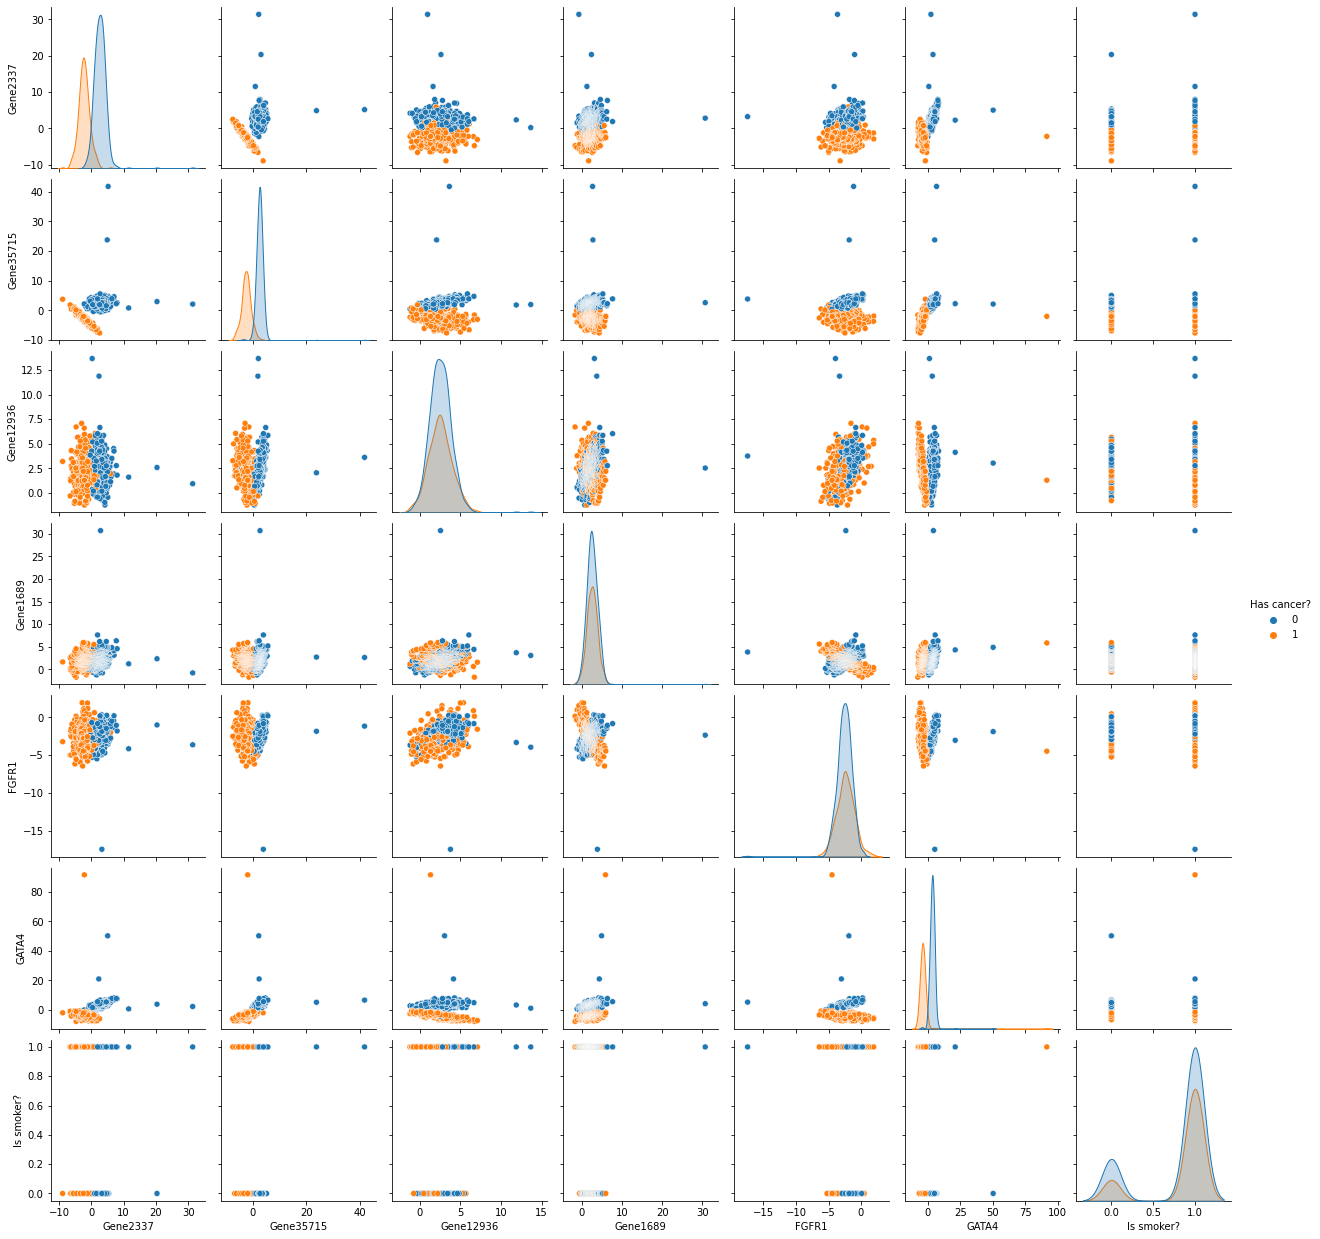
\includegraphics[scale=0.35]{pair0}
\end{center}\pagebreak

Построю корреляционную матрицу для признаков:
\begin{center}
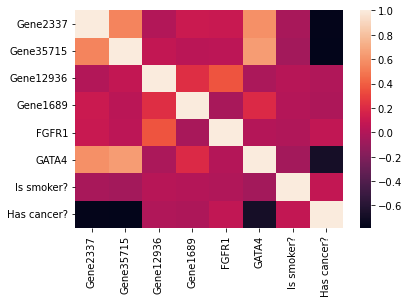
\includegraphics[scale=0.65]{corr0}
\end{center}
Так же построю гистограммы для числовых признаков:
\begin{center}
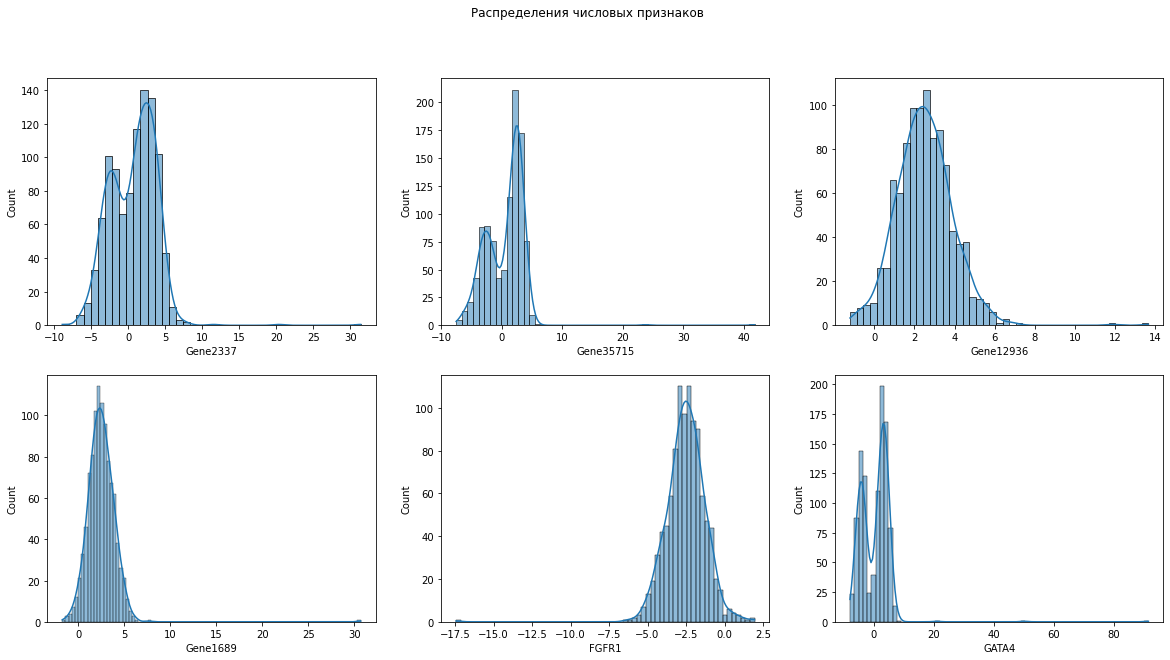
\includegraphics[scale=0.35]{bar0}
\end{center}
Видно, что в данных присутствуют выбросы, которые могут повлиять на обучение модели. Числовые данные не превосходят по модулю $10$, поэтому удалю все элементы, в которых это правило не соблюдается.
\pagebreak

Теперь ничего не мешает анализу. Построю те же графики для обработанного набора данных:
\begin{center}
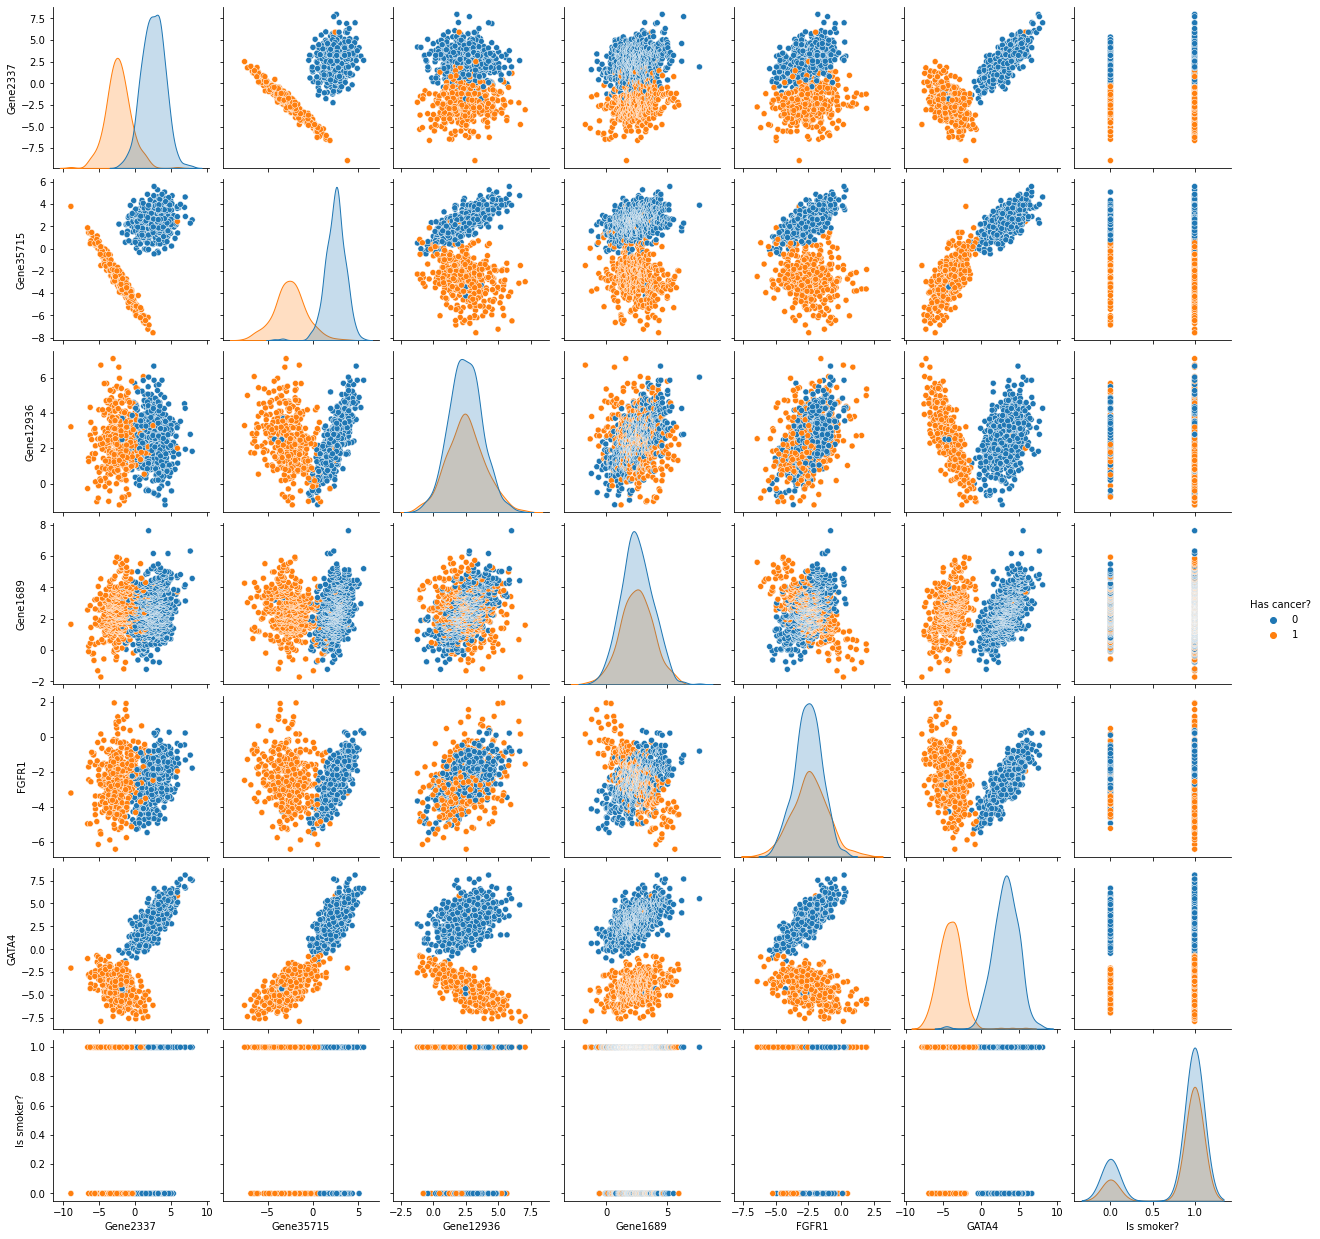
\includegraphics[scale=0.35]{pair1}
\end{center}
Исходя из парных графиков, можно сделать вывод, что задачу реально решить линейной моделью: на большинстве рисунков можно довольно точно провести прямую, разделяющую синие и оранжевые точки.
\pagebreak

Корреляционная матрица после удаления выбросов не изменилась:
\begin{center}
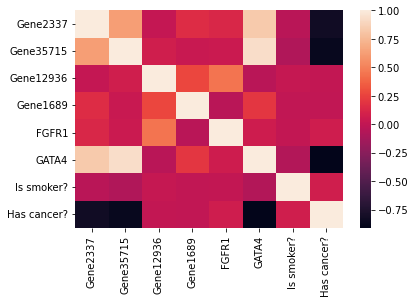
\includegraphics[scale=0.65]{corr1}
\end{center}
Видно, что больше всего на результат влияют <<Gene2337>>, <<Gene35715>> и <<GATA4>>, которые ещё и довольно сильно коррелируют между собой. <<Gene12936>>, <<Gene1689>>, <<FGFR1>> и фактор курения влияют меньше.

Гистограммы распределения числовых признаков:
\begin{center}
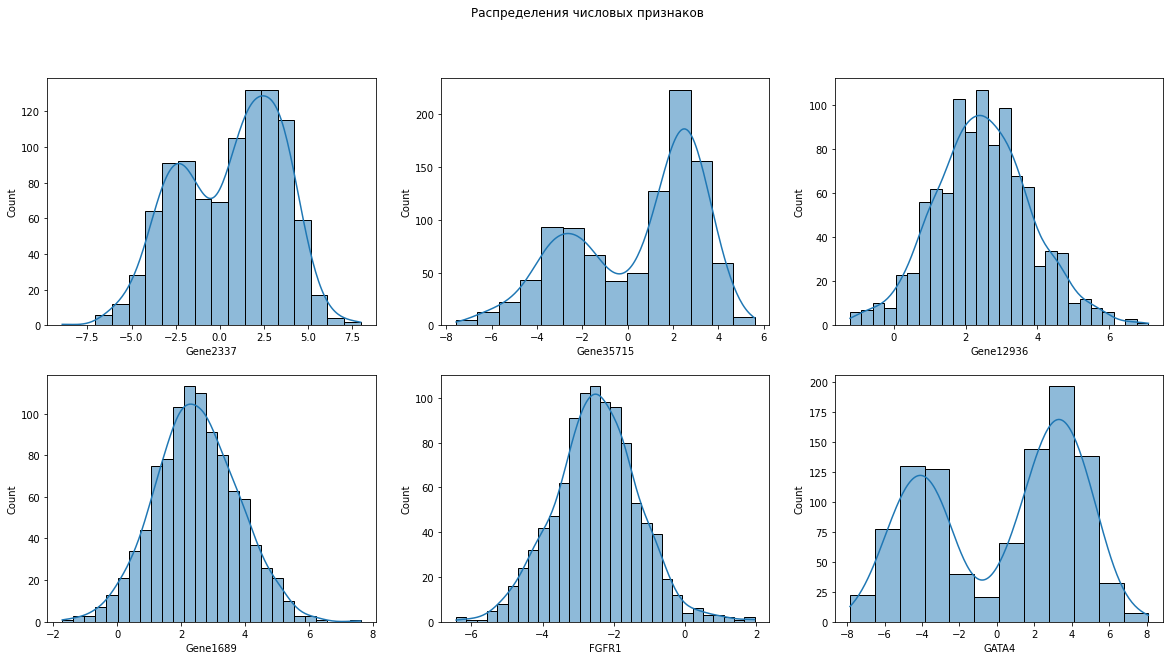
\includegraphics[scale=0.35]{bar1}
\end{center}
Полученных данных достаточно для построения модели, об этом говорят попарные графики и корреляционная матрица. Добавление новых признаков не требуется.

\pagebreak

Соотношение классов объектов:
\begin{center}
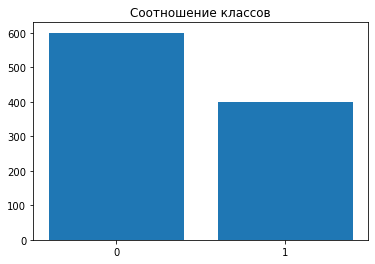
\includegraphics[scale=0.65]{classes}
\end{center}
Объектов разных классов примерно одинаковое количество, oversampling не требуется. Данные готовы к обучению.

\pagebreak
